\documentclass[a4paper,12pt]{article}

%%% Работа с русским языком
\usepackage{cmap}					% поиск в PDF
\usepackage{mathtext} 				% русские буквы в формулах
\usepackage[T2A]{fontenc}			% кодировка
\usepackage[utf8]{inputenc}			% кодировка исходного текста
\usepackage[english,russian]{babel}	% локализация и переносы
\usepackage{indentfirst}            % красная строка в первом абзаце
\usepackage{extarrows}              % длинное равно
\frenchspacing                      % равные пробелы между словами и предложениями

%%% Дополнительная работа с математикой
\usepackage{amsmath,amsfonts,amssymb,amsthm,mathtools} % пакеты AMS
\usepackage{icomma}                                    % "Умная" запятая
\usepackage{physics} % для символа нормы

%%% Свои символы и команды
\usepackage{centernot} % центрированное зачеркивание символа
\usepackage{stmaryrd}  % некоторые спецсимволы

\usepackage{pythonhighlight}

% \renewcommand{\epsilon}{\ensuremath{\varepsilon}}
% \renewcommand{\phi}{\ensuremath{\varphi}}
% \renewcommand{\kappa}{\ensuremath{\varkappa}}
% \renewcommand{\le}{\ensuremath{\leqslant}}
% \renewcommand{\leq}{\ensuremath{\leqslant}}
% \renewcommand{\ge}{\ensuremath{\geqslant}}
% \renewcommand{\geq}{\ensuremath{\geqslant}}
% \renewcommand{\emptyset}{\ensuremath{\varnothing}}

% \DeclareMathOperator*{\Mid}{\scalebox{1.1}{$\mid$}}
\DeclareMathOperator*{\argmax}{argmax}

% \DeclareMathOperator{\sgn}{sgn}
% \DeclareMathOperator{\gd}{\text{НОД}}
% \DeclareMathOperator{\lf}{\text{НОК}}
% \DeclareMathOperator{\rk}{rk}
% \DeclareMathOperator{\pr}{pr}
% \DeclareMathOperator{\im}{Im}
% \DeclareMathOperator{\ke}{Ker}
% \DeclareMathOperator{\re}{Re}
% \DeclareMathOperator{\cha}{char}
% \DeclareMathOperator{\ord}{ord}
% \DeclareMathOperator{\tr}{tr}
% \DeclareMathOperator{\md}{mod}
% \DeclareMathOperator{\Aut}{Aut}
% \DeclareMathOperator{\Inn}{Inn}
% \DeclareMathOperator{\End}{End}
% \DeclareMathOperator{\GL}{GL}
% \DeclareMathOperator{\SL}{SL}
% \DeclareMathOperator{\diag}{diag}

\newcommand{\divby}{
	\mathrel{\vbox{\baselineskip.65ex\lineskiplimit0pt\hbox{.}\hbox{.}\hbox{.}}}
}
\newcommand{\notdivby}{\centernot\divby}
% \newcommand\norm[1]{\left\lVert#1\right\rVert}
% \newcommand\normx[1]{\left\Vert#1\right\Vert}
\newcommand{\N}{\mathbb{N}}
\newcommand{\Z}{\mathbb{Z}}
\newcommand{\Q}{\mathbb{Q}}
\newcommand{\R}{\mathbb{R}}
\newcommand{\E}{\mathbb{E}}
\newcommand{\D}{\mathbb{D}}
\newcommand{\Cm}{\mathbb{C}}
\newcommand{\F}{\mathbb{F}}
\newcommand{\id}{\mathrm{id}}
\newcommand{\imp}[2]{(#1\,\,$\ra$\,\,#2)\,\,}
\newcommand{\nset}[1]{\{1, \dotsc, #1\}}
\newcommand{\Chi}{\scalebox{1.1}{\raisebox{\depth}{$\chi$}}}
\newcommand{\FF}{\scalebox{0.95}{$\mathcal F$}}
\newcommand{\FFF}{\scalebox{0.55}{$\mathcal F$}}
\newcommand{\GG}{\scalebox{0.95}{$\mathcal G$}}
\newcommand{\GGG}{\scalebox{0.55}{$\mathcal G$}}

\newcommand{\ND}[2]{\mathcal{N}\left({#1}, {#2}\right)} % normal distribution
\newcommand{\tod}{\xrightarrow[]{d}}
\newcommand{\toP}{\xrightarrow[]{P}}
\newcommand{\tolp}[1]{\xrightarrow[]{L_{#1}}}
\newcommand{\toac}{\xrightarrow[]{\text{п. н.}}} % almost certainly

\renewcommand\labelitemi{$\triangleright$}
\newcommand{\LL}{\mathcal{L}}
\newcommand{\todo}[1]{\textcolor{red}{TODO} #1}
\let\bs\backslash
\let\vect\overline
\let\normal\trianglelefteqslant
\let\lra\Leftrightarrow
\let\ra\Rightarrow
\let\la\Leftarrow
\let\gl\langle
\let\gr\rangle
\let\sd\leftthreetimes
\let\emb\hookrightarrow
\let\mc\mathcal
\let\mf\mathfrak

%%% Перенос знаков в формулах (по Львовскому)
\newcommand*{\hm}[1]{#1\nobreak\discretionary{}{\hbox{$\mathsurround=0pt #1$}}{}}
\renewcommand{\phi}{\varphi}
\newcommand{\eps}{\varepsilon}

%%% Работа с картинками
\usepackage{graphicx}    % Для вставки рисунков
\setlength\fboxsep{3pt}  % Отступ рамки \fbox{} от рисунка
\setlength\fboxrule{1pt} % Толщина линий рамки \fbox{}
\usepackage{wrapfig}     % Обтекание рисунков текстом

%%% Работа с таблицами
\usepackage{array,tabularx,tabulary,booktabs} % Дополнительная работа с таблицами
\usepackage{longtable}                        % Длинные таблицы
\usepackage{multirow}                         % Слияние строк в таблице

%%% Теоремы
\theoremstyle{definition}
\newtheorem{problem}{}
\newtheorem{theorem}{Теорема}
\newtheorem*{lemma}{Лемма}
% \newtheorem{proposition}{Утверждение}[section]
% \newtheorem*{exercise}{Упражнение}
% \newtheorem{problem}{}

% \theoremstyle{definition}
% \newtheorem{definition}{Определение}[section]
% \newtheorem*{corollary}{Следствие}
% \newtheorem*{note}{Замечание}
% \newtheorem*{reminder}{Напоминание}
% \newtheorem*{example}{Пример}

\theoremstyle{remark}
\newtheorem*{solution}{Решение}
\newtheorem*{guidance}{Указание}
\newtheorem*{prooff}{Д-во}

%%% Оформление страницы
\usepackage{extsizes}     % Возможность сделать 14-й шрифт
\usepackage{geometry}     % Простой способ задавать поля
\usepackage{setspace}     % Интерлиньяж
\usepackage{enumitem}     % Настройка окружений itemize и enumerate
\setlist{leftmargin=25pt} % Отступы в itemize и enumerate

\geometry{top=25mm}    % Поля сверху страницы
\geometry{bottom=30mm} % Поля снизу страницы
\geometry{left=20mm}   % Поля слева страницы
\geometry{right=20mm}  % Поля справа страницы

\setlength\parindent{15pt}                % Устанавливает длину красной строки 15pt
\linespread{1.3}                          % Коэффициент межстрочного интервала
%\setlength{\abovedisplayskip}{3pt}       % Отступы от выключных формул
%\setlength{\belowdisplayskip}{3pt}       % Отступы от выключных формул
%\setlength{\abovedisplayshortskip}{3pt}  % Отступы от выключных формул
%\setlength{\abovedisplayshortskip}{3pt}  % Отступы от выключных формул
%\setlength{\parskip}{0.5em}              % Вертикальный интервал между абзацами
%\setcounter{secnumdepth}{0}              % Отключение нумерации разделов
%\setcounter{section}{-1}                 % Нумерация секций с нуля
\usepackage{multicol}			          % Для текста в нескольких колонках
\usepackage{soulutf8}                     % Модификаторы начертания

%%% Содержаниие
\usepackage{tocloft}
\renewcommand{\thesection}{\arabic{section}.} 
\renewcommand{\thesubsection}{\thesection.\arabic{subsection}.}
\tocloftpagestyle{main}
%\setlength{\cftsecnumwidth}{2.3em}
%\renewcommand{\cftsecdotsep}{1}
%\renewcommand{\cftsecpresnum}{\hfill}
%\renewcommand{\cftsecaftersnum}{\quad}

%%% Шаблонная информация для титульного листа
\newcommand{\CourseName}{Математическая статистика}
\newcommand{\FullCourseName}{\so{МАТЕМАТИЧЕСКАЯ СТАТИСТИКА}}
\newcommand{\TaskNumber}{II}
\newcommand{\CourseDate}{весна 2024}
\newcommand{\AuthorInitials}{Яфаров Руслан}

%%% Колонтитулы
% \usepackage{titleps}
% \newpagestyle{main}{
% 	\setheadrule{0.4pt}
% 	\sethead{\CourseName}{}{\hyperlink{intro}{\;Назад к содержанию}}
% 	\setfootrule{0.4pt}                       
% 	\setfoot{ФПМИ МФТИ, \CourseDate}{}{\thepage} 
% }
% \pagestyle{main}  

%%% Нумерация уравнений
\makeatletter
\def\eqref{\@ifstar\@eqref\@@eqref}
\def\@eqref#1{\textup{\tagform@{\ref*{#1}}}}
\def\@@eqref#1{\textup{\tagform@{\ref{#1}}}}
\makeatother                      % \eqref* без гиперссылки
\numberwithin{equation}{section}  % Нумерация вида (номер_секции).(номер_уравнения)
\mathtoolsset{showonlyrefs=false} % Номера только у формул с \eqref{} в тексте.

%%% Гиперссылки
\usepackage{hyperref}
% \usepackage[usenames,dvipsnames,svgnames,table,rgb]{xcolor}
\hypersetup{
	unicode=true,            % русские буквы в раздела PDF
	colorlinks=true,       	 % Цветные ссылки вместо ссылок в рамках
	linkcolor=black!15!blue, % Внутренние ссылки
	citecolor=green,         % Ссылки на библиографию
	filecolor=magenta,       % Ссылки на файлы
	urlcolor=NavyBlue,       % Ссылки на URL
}

%%% Графика
\usepackage{tikz}        % Графический пакет tikz
\usepackage{tikz-cd}     % Коммутативные диаграммы
\usepackage{tkz-euclide} % Геометрия
\usepackage{stackengine} % Многострочные тексты в картинках

\begin{document}
	\begin{titlepage}
	\clearpage\thispagestyle{empty}
	\centering
	
	\textbf{Московский физико-технический институт}
	\vspace{33ex}
	
	{\textbf{\FullCourseName}}
	
	\TaskNumber\ ЗАДАНИЕ 
	\vspace{1ex}

	\begin{flushright}
		\noindent
		Автор: {\AuthorInitials},
		\\
		Б13-202 
	\end{flushright}
	
	\vfill
	\CourseDate
	\pagebreak
\end{titlepage}
	\section{Случайные величины и их характеристики}
	\problem{~
	\begin{center} 
	    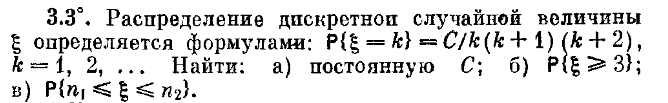
\includegraphics[width=\textwidth]{1.png}
	\end{center}
	}
	\solution{~
	\begin{enumerate}[label=\alph*]
		\item \[\sum_{k = 1}^{\infty} \frac{1}{k(k + 1)(k + 2)} = \sum_{k = 1}^{\infty} \frac{1}{k}\left(\frac{1}{k + 1} - \frac{1}{k + 2}\right) = \sum_{k = 1}^{\infty} \left(\frac{1}{2}\left(\frac{1}{k} - \frac{1}{k + 1}\right) - \frac{1}{2}\left(\frac{1}{k + 1} - \frac{1}{k + 2}\right)\right) = \]$\frac{1}{2} - \frac{1}{4} = \frac{1}{4}$. Имеем $\frac{C}{4} = 1 \ra C = 4$.
		\item $P(\xi \ge 3) = 1 - P(\xi < 3) = 1 - (P(\xi = 1) + P(\xi = 2)) = \frac{1}{6}$. 
		\item $P(n_1 \le \xi \le n_2) = \frac{1}{2}\left(\frac{1}{n_1} - \frac{1}{n_2} - \frac{1}{n_1 + 1} + \frac{1}{n_2 + 1}\right) = \frac{1}{2}\left(\frac{1}{n_1(n_1 + 1)} - \frac{1}{n_2(n_2 + 1)}\right)$
	\end{enumerate}
	}
	\problem{~
	\begin{center} 
	    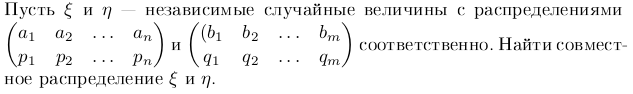
\includegraphics[width=\textwidth]{2.png}
	\end{center}
	}
	\solution{
	$P(\xi = a_i, \eta = b_j) = p_iq_j$
	}
	\problem{~
	\begin{center} 
	    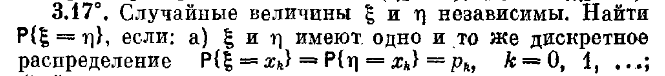
\includegraphics[width=\textwidth]{3.png}
	\end{center}
	}
	\solution{
	$P(\xi = \eta) = \sum_{k = 0}^{\infty} P(\xi = x_k, \eta = x_k) = \sum_{k = 0}^{\infty} p_k^2$
	}
	\problem{~
	\begin{center} 
	    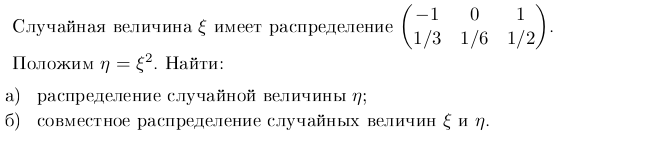
\includegraphics[width=\textwidth]{4.png}
	\end{center}
	}
	\solution{~
	\begin{enumerate}[label=\alph*]
	\item $P(\eta = 1) = \frac{5}{6}, P(\eta = 0) = \frac{1}{6}$
	\item $P(\xi = -1, \eta = 1) = \frac{1}{3}, P(\xi = 0, \eta = 0) = \frac{1}{6}, P(\xi = 1, \eta = 1) = \frac{1}{2}$
    \end{enumerate}
	}
	\problem{~
	\begin{center} 
	    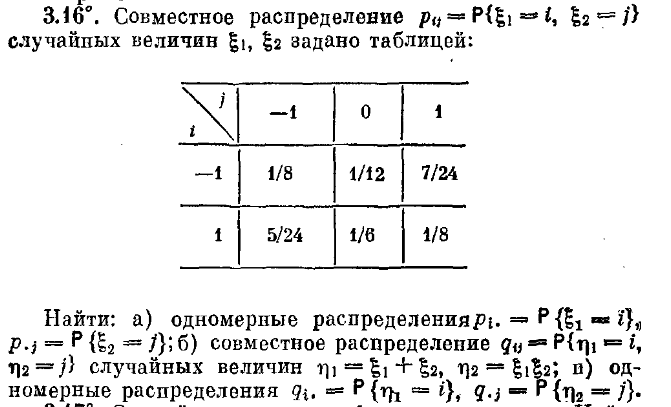
\includegraphics[width=\textwidth]{5.png}
	\end{center}
	}
	\solution{~
	\begin{enumerate}[label=\alph*]
		\item $p_{i\cdot} = \sum_j p_{ij}, p_{\cdot j} = \sum_i p_{ij}$. $p_{-1\cdot} = \frac{1}{2}, p_{1\cdot} = \frac{1}{2}, p_{\cdot-1} = \frac{1}{3}, p_{\cdot0} = \frac{1}{4}, p_{\cdot1} = \frac{5}{12}$
		\item $q_{-21} = \frac{1}{8}, q_{-10} = \frac{1}{12}, q_{10} = \frac{1}{6}, q_{21} = \frac{1}{8}, q_{0-1} = \frac{1}{2}$
		\item $q_{-2\cdot} = q_{-21}, q_{-1\cdot} = q_{-10}, q_{0\cdots} = q_{0-1}, q_{1\cdot} = q_{10}, q_{2\cdot} = q_{21}, q_{\cdot-1} = q_{0-1}, q_{\cdot0} = \frac{1}{4}, q_{\cdot1} = \frac{1}{4}$
	\end{enumerate}
	}
	\problem{~
	\begin{center} 
	    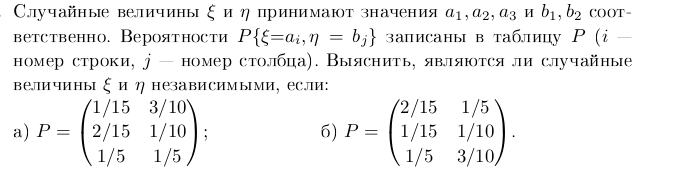
\includegraphics[width=\textwidth]{6.png}
	\end{center}
	}
	\solution{~
	\begin{enumerate}[label=\alph*]
		\item $P(\xi = a_1) = \frac{11}{30}, P(\eta = b_1) = \frac{2}{5}, P(\xi = a_1, \eta = b_1) = \frac{1}{15} \ne P(\xi = a_1)P(\eta = b_1) = \frac{11}{75} \ra $ Нет, не являются.
		\item $P(\xi = a_1) = \frac{1}{3}, P(\xi = a_2) = \frac{1}{6}, P(\xi = a_3) = \frac{1}{2}, P(\eta = b_1) = \frac{2}{5}, P(\eta = b_2) = \frac{3}{5}$ Являются. 
	\end{enumerate}
	}
	\problem{~
	\begin{center} 
	    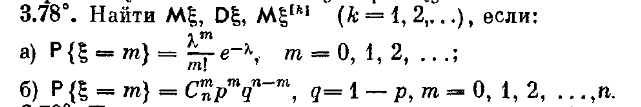
\includegraphics[width=\textwidth]{7.png}
	\end{center}
	(Найти только математическое ожидание и дисперсию)
	}
	\solution{~
	\begin{enumerate}[label=\alph*]
		\item \[\E\xi = \sum_{m = 1}^{\infty} \frac{\lambda^m}{(m - 1)!}e^{-\lambda} = \lambda e^{-\lambda} \sum_{m = 0}^{\infty} \frac{\lambda^m}{m!} = \lambda, \text{ } \E\xi(\xi - 1) = e^{-\lambda} \sum_{m = 0}^{\infty} m(m - 1) \frac{\lambda^m}{m!} = \lambda^2e^{-\lambda} \sum_{m = 2}^{\infty} \frac{\lambda^{m - 2}}{(m - 2)!}\] $ = \lambda^2 = \E\xi^2 - \E\xi \ra \E\xi^2 = \lambda^2 + \lambda \ra \D\xi = \E\xi^2 - (\E\xi)^2 = \lambda$
		\item \[\xi = \sum_{i = 1}^n \xi_i, \xi_i \sim Bern(p), \xi_i \text{ независимы } \ra \E\xi = \sum_{i = 1}^n \E\xi_i = np. \text{ }\D \xi = \sum_{i = 1}^n \D \xi_i = npq\]
	\end{enumerate}
	}
	\problem{~
	\begin{center} 
	    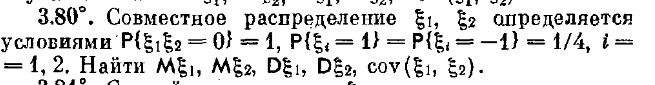
\includegraphics[width=\textwidth]{8.png}
	\end{center}
	}
	\solution{
	$P(\xi_1 \ne 0) \ge \frac{1}{2} \ra P(\xi_2 = 0) \ge \frac{1}{2}$(от противного доказывается очевидно). $P(\xi_2 = 0) > \frac{1}{2} $ быть не может так как тогда $\sum_{a_i} P(\xi = a_i) > 1 \ra P(\xi_1 = 0) = P(\xi_2 = 0) = \frac{1}{2}\text{ }\E \xi_1 = \E \xi_2 = 0\text{ } \D \xi_1 = \D \xi_2 = \frac{1}{2}. \cov(\xi_1, \xi_2) = \E\xi_1\xi_2 = 0$
	}
	\problem{~
	\begin{center} 
	    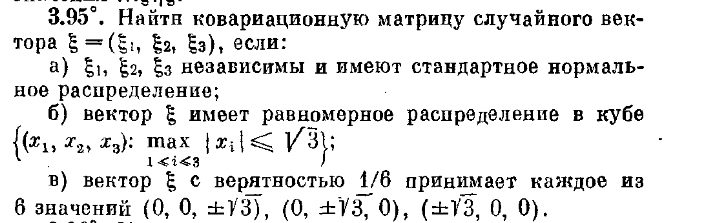
\includegraphics[width=\textwidth]{9.png}
	\end{center}
	}
	\solution{~
\begin{enumerate}[label=\alph*]
		\item $\cov \xi = E$
		\item \[\D x_i = \int_{-\sqrt 3}^{\sqrt3} x^2dx = \left. \frac{x^3}{3} \right\vert_{-\sqrt 3}^{\sqrt 3} = 2\sqrt 3 \ra \text{ так как $x_i$ независимы } \cov \xi = 2\sqrt3 E\]
		\item $\E x_i = 0 \ra \D x_i = \E x_i^2 = 3 * \frac{1}{3} = 1$. $x_ix_j = 0 \forall i \ne j \ra cov \xi = E$ 
	\end{enumerate}
	}
	\problem{~
	\begin{center} 
	    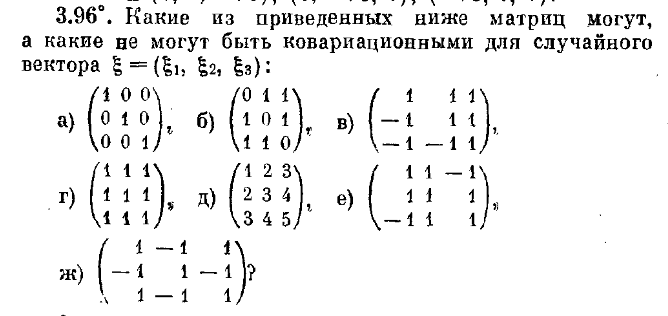
\includegraphics[width=\textwidth]{10.png}
	\end{center}
	}
	\solution{~
	\begin{enumerate}[label=\alph*]
	    \item Может, пример выше
	    \item Не может, $\D \eta = 0 \ra \eta = const$, а значит $\eta - \E \eta = 0 \ra cov( \xi_i, \xi_j) = 0$.
	    \item Не может, так как она не симментрична
	    \item Ну, вроде может
	    \item Не может, так как она не положительно полуопределена
	    \item не положительно полуопределена
	    \item Ну, вроде может
\end{enumerate}
	}
	\problem{~
	\begin{center} 
	    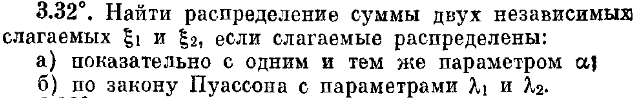
\includegraphics[width=\textwidth]{11.png}
	\end{center}
	(б)
	}
	\solution{~
	\[P(\xi = m) = \sum_{k = 0}^m P(\xi_1 = k)P(\xi_2 = m - k) = \sum_{k = 0}^m \frac{\lambda_1^k}{k!}e^{-\lambda_1}\frac{\lambda_2^{m - k}}{(m - k)!}e^{-\lambda_2} = \frac{e^{-(\lambda_1 + \lambda_2)}}{m!}\sum_{k = 0}^m C_m^k\lambda_1^k\lambda_2^{m - k}\] \[=\frac{(\lambda_1 + \lambda_2)^m}{m!}e^{-(\lambda_1 + \lambda_2)}\]
	}
	\problem{~
	\begin{center} 
	    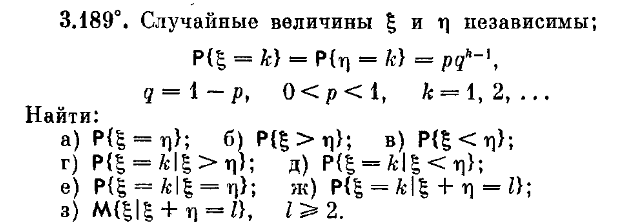
\includegraphics[width=\textwidth]{12.png}
	\end{center}
	(а, б, в)
	}
	\solution{~
	\begin{enumerate}[label=\alph*]
		\item $P(\xi = \eta) = \sum_{k = 1}^{\infty} (pq^{k - 1})^2 = p^2q^{-2} \sum_{k = 1}^{\infty} q^{2k} = p^2q^{-2}\frac{q^2}{1 - q^2} = \frac{p^2}{1 - q^2}$
		\item Из сооброжений симметрии $P(\xi > \eta) = P(\eta > \xi) = p$. $2p + P(\xi = \eta) = 1 \ra p = \frac{1}{2}\left(1 - \frac{p^2}{1 - q^2} \right)$
	\end{enumerate}
	}
	\problem{~
	\begin{center} 
	    
\includegraphics[width=\textwidth]{13.png}
	\end{center}
	}
	\solution{
	Пусть вероятность вынуть белый шар равна $p = \frac{m}{m + n}$, черный - $q = 1 - p$. Тогда $\xi - $ случайная величина, равная кол-ву вынутых шаров. $P(\xi = k) = q^{k - 1}p$. Рассмотрим функцию $f(x) = \displaystyle \sum_{k = 1}^{\infty} x^k = \frac{x}{1 - x}. f'(x) = \frac{1}{(1 - x)^2} = \sum_{k = 1}^{\infty} kx^{k - 1}. f''(x) = \frac{-2(x - 1)}{(x - 1)^4} = \frac{2}{(1 - x)^3} = \sum_{k = 0}^{\infty} k(k - 1)x^{k - 2} \ra \E\xi = \sum_{k = 1}^{\infty}pq^{k - 1}k = pf'(q) = \frac{p}{(1 - q)^2} = \frac{1}{p} = 1 + \frac{n}{m}. \E \xi(\xi - 1) = \sum_{k = 1}^{\infty}pq^{k - 1}k(k - 1) = qpf''(q) = \frac{2qp}{p^3} = \frac{2q}{p^2} \ra \E\xi^2 = \frac{2q}{p^2} + \frac{1}{p} = \frac{2q + p}{p^2} \ra \D\xi = \frac{2q + p}{p^2} - \frac{1}{p^2} = \frac{1 - p}{p^2} = \frac{q}{p^2} = \frac{n}{m}\left(1 + \frac{n}{m} \right)$
	}
	\section{Схема Бернулли: закон больших чисел, предельные теоремы Пуассона и Муавра-Лапласа}
	\problem{~
	\begin{center} 
	    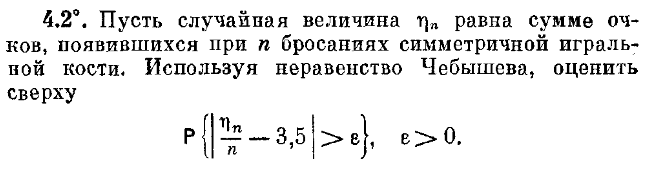
\includegraphics[width=\textwidth]{14.png}
	\end{center}
	}
	\solution{
	$\eta_n = \sum_{i = 1}^n \xi_i$, где $\xi_i - $ сл-я величина очков одного броска кубика, оч-но $\xi_i$ независимы. $\E \xi_i = \frac{7}{2}, \D\xi = \frac{35}{12} \ra \E\eta_n = n\frac{7}{2}, \D \eta_n = n\frac{35}{12}$. По неравенству Чебышева $P(\left|\frac{\eta_n}{n} - 3.5\right| > \eps) = P(\left|\eta_n - 3.5n \right|> n\eps) = P(\left|\eta_n - \E\eta_n\right| > n\eps) \le \frac{\D \eta_n}{n^2\eps^2} = \frac{35}{12n\eps^2}$
	}
	\problem{~
	\begin{center} 
	    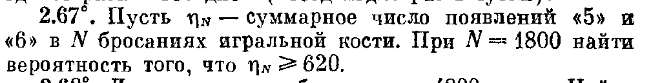
\includegraphics[width=\textwidth]{15.png}
	\end{center}
	}
	\solution{
	$\eta_N \sim Bin(N, \frac{1}{3}) \ra \E \eta_N = \frac{N}{3} = 600, \D \eta_N = \frac{2N}{9} = 400$ По интегральной теореме Муавра-Лапласа $P(\eta_N \ge 620) = \displaystyle \int_{\frac{620 - 600}{\sqrt{400}}}^{+\infty} \frac{1}{\sqrt{2\pi}}e^{-\frac{x^2}{2}}dx = 1 - \Phi(1) \approx 0.1587$
	}
	\problem{~
	\begin{center} 
	    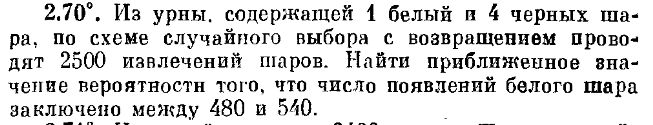
\includegraphics[width=\textwidth]{16.png}
	\end{center}
	}
	\solution{
	$\xi \sim Bin(2500, \frac{1}{5}) \E\xi = 500, \D \xi = 400, P(480 \le \xi \le 540) = P(\frac{480 - 500}{\sqrt{400}} \le \frac{\xi - \E\xi}{\sqrt{\D\xi}} \le \frac{540 - 500}{\sqrt{400}}) = P(-1 \le \overset{*}{\xi} \le 2) = \Phi(2) - \Phi(-1) \approx 0.8185$
	}
	\problem{~
	\begin{center} 
	    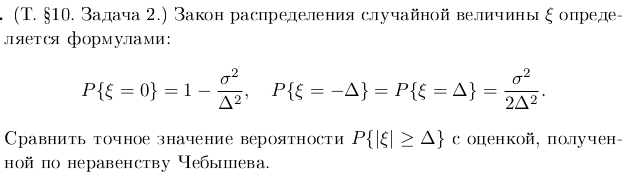
\includegraphics[width=\textwidth]{17.png}
	\end{center}
	}
	\solution{
	$\E\xi = 0, \E\xi^2 = \sigma^2 \ra \D\xi = \sigma^2, P(|\xi| \ge \Delta) \le \frac{\sigma^2}{\Delta^2}$. Они равны, емае...
	}
	\problem{~
	\begin{center} 
	    
\includegraphics[width=\textwidth]{18.png}
	\end{center}
	}
	\solution{~}
	\problem{~
	\begin{center} 
	    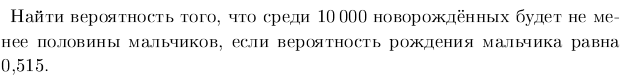
\includegraphics[width=\textwidth]{19.png}
	\end{center}
	}
	\solution{
	$\xi \sim Bin(N, p) P(\xi \ge \frac{N}{2}) = \displaystyle \int_{\frac{\frac{N}{2} - Np}{\sqrt{Np(1 - p)}}}^{+\infty}\frac{1}{\sqrt{2\pi}}e^{-\frac{x^2}{2}}dx = 1 - \Phi\left(\sqrt{\frac{N}{p(1 - p)}}\left(\frac{1}{2} - p\right)\right) = 1 - \Phi\left(\sqrt{\frac{10000}{0.515 * 0.485}}\left(-0.015\right)\right) \approx 1 - \Phi(-0.94911) \approx 0.8289$
	}
	\section{Случайная величина в общей теоретико вероятностной схеме. Характеристические и производящие функции. Центральная предельная теорема}
	\problem{~
	\begin{center} 
	    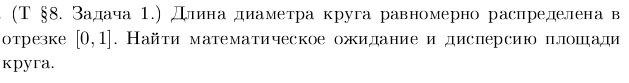
\includegraphics[width=\textwidth]{20.png}
	\end{center}
	}
	\solution{
	$\E(\frac{\pi\xi^2}{4}) = \displaystyle \frac{1}{4}\int_{\R}\pi x^2 I_{x \in [0,1]}dx = \frac{\pi}{12}. \E\left(\frac{\pi\xi^2}{4}\right)^2 = \frac{1}{16}\int_{\R}\pi^2 x^4 I_{x \in [0,1]}dx = \frac{\pi^2}{80} \ra \D\left(\frac{\pi\xi^2}{4}\right) = \frac{\pi^2}{80} - \frac{\pi^2}{144} = \frac{\pi^2}{180}$
	}
	\problem{~
	\begin{center} 
	    
\includegraphics[width=\textwidth]{21.png}
	\end{center}
	}
	\solution{
	По теореме об обратной функции $\exists F^{-1}(x)$. Тогда $F_{\eta}(y) = P(\eta \le y) = P(F(\xi) \le y) = P(\xi \le F^{-1}(y)) = F_{\xi}(F^{-1}(y))$
	}
	\problem{~
	\begin{center} 
	    
\includegraphics[width=\textwidth]{22.png}
	\end{center}
	}
	\solution{~
	\[F_{\eta}(x) = P(\min_{1 \le i \le n} \xi_i \le x) = 1 - P(\min_{1 \le i \le n} \xi_i > x) = 1 - \prod_{i = 1}^n P(\xi_i > x) = 1 - \prod_{i = 1}^n (1 - F_{\xi_i}(x))\]
	\[F_{\zeta}(x) = \prod_{i = 1}^n F_{\xi_i}(x)\]
	}
	\problem{~
	\begin{center} 
	    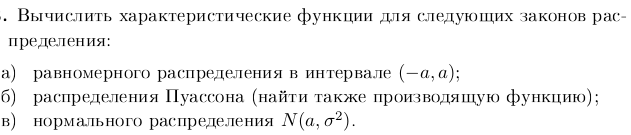
\includegraphics[width=\textwidth]{23.png}
	\end{center}
	}
	\solution{~
	\begin{enumerate}[label=\alph*]
	\item $\xi \sim R(-a, a)$
	\[\psi_{\xi}(t) = \E e^{it\xi} = \E \cos t\xi + i\E \sin t\xi = \int_{-a}^a \cos tx \frac{1}{2a}dx + i\int_{-a}^a \sin tx \frac{1}{2a}dx = \begin{cases} \left. -\frac{\sin tx}{2ta} = \right|_{-a}^{a} = -\frac{\sin ta}{ta}, t \ne 0 \\ 1, t = 0 \end{cases}\]
	\item $\xi \sim Pois(\lambda)$
	\[\psi_{\xi}(t) = \sum_{k = 0}^{\infty} e^{itk}\frac{\lambda^k}{k!}e^{-\lambda} = e^{-\lambda} \sum_{k = 0}^{\infty}\frac{(e^{it}\lambda)^k}{k!} = e^{\lambda(e^{it} - 1)}\]
	\item $\xi \sim N(a, \sigma^2)$
	\[\psi_{\xi}(t) = \int_{-\infty}^{+\infty} e^{itx} \frac{1}{\sqrt{2\pi\sigma^2}}e^{-\frac{(x - a)^2}{2\sigma^2}}dx = \frac{1}{\sigma \sqrt{2\pi}}\int_{-\infty}^{+\infty} e^{-\frac{1}{2}\left(\left(\frac{x - a}{\sigma} -\sigma ti\right)^2 - 2ati + \sigma^2t^2\right)} dx = \]
	\[\frac{e^{ati - \frac{\sigma^2t^2}{2}}\sigma}{\sigma\sqrt{2\pi}} \int_{-\infty}^{+\infty} e^{\frac{\left(\frac{x - a}{\sigma} -\sigma ti\right)^2}{2}}d\left(\frac{x - a}{\sigma} -\sigma ti\right) = e^{ati - \frac{\sigma^2t^2}{2}} \frac{\int_{-\infty}^{+\infty} e^{-\frac{u^2}{2}}du}{\sqrt{2\pi}} = e^{ati - \frac{\sigma^2t^2}{2}}\]
\end{enumerate}
	}
	\problem{~
	\begin{center} 
	    
\includegraphics[width=\textwidth]{24.png}
	\end{center}
	}
	\solution{~
	\begin{enumerate}[label=\alph*]
	\item $\cos t = \frac{e^{it} + e^{-it}}{2} = e^{it * 1}\frac{1}{2} + e^{it(-1)}\frac{1}{2} \ra \xi \sim 
	\begin{pmatrix}
	1 & -1 \\
	\frac{1}{2} & \frac{1}{2}
	\end{pmatrix}$
	\item $e^{it}\cos t = \cos^2t + i\sin t\cos t = \frac{1}{2} + \frac{\cos 2t}{2} + i\frac{\sin 2t}{2} = \frac{e^{it*0}}{2} + \frac{e^{it*2}}{2} \ra \xi \sim
	\begin{pmatrix}
	0 & 2 \\
	\frac{1}{2} & \frac{1}{2}
	\end{pmatrix} $
	\item $\frac{1}{2 - e^{it}} = \frac{1}{2}\sum_{k = 0}^{\infty} \frac{e^{itk}}{2^k} = \sum_{k = 0}^{\infty} \frac{e^{itk}}{2^{k + 1}} \ra P(\xi = k) = \frac{1}{2^{k + 1}} \forall k = 0, 1, \cdots $
\end{enumerate}
	}
	\problem{~
	\begin{center} 
	    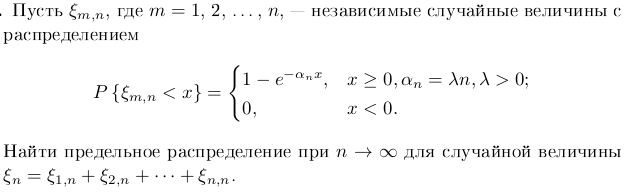
\includegraphics[width=\textwidth]{25.png}
	\end{center}
	}
	\solution{
	$P(\xi_{m, n} < x) = F(x) \ra \frac{dF}{dx} = p(x) = 
	\begin{cases}
	\alpha_ne^{-\alpha_nx}, x \ge 0 \\
	0, x < 0
	\end{cases} \ra \E \xi_{m, n} = \int_{0}^{+\infty} p(x)xdx = \int_{0}^{+\infty}\alpha_ne^{-\alpha_nx}xdx = -\int_{0}^{+\infty}xd(e^{-\alpha_nx}) = -(\left.xe^{-\alpha_nx}\right|_{0}^{+\infty} - \int_{0}^{+\infty}e^{-\alpha_nx}dx) = \left.\frac{e^{-\alpha_nx}}{-\alpha_n}\right|_{0}^{+\infty} = \frac{1}{\alpha_n}\\
	\E\xi_{m, n}^2 = \int_{0}^{+\infty}p(x)x^2dx = -(\left.x^2e^{-\alpha_nx}\right|_{0}^{+\infty} - 2\int_{0}^{+\infty}xe^{-\alpha_nx}dx) = \frac{2}{\alpha_n^2} \ra \D \xi_{m, n} = \frac{1}{\alpha_n^2} \ra \frac{\xi_n - n\E\xi_{m, n}}{\sqrt{n\D\xi_{m, n}}} =  \sqrt{n}\frac{\xi_n - \frac{1}{\lambda}}{\frac{1}{\lambda}} = \sqrt{n}(\lambda \xi_n - 1)$
	}
	\section{Условное математическое ожидание}
	\problem{~
	\begin{center} 
	    
\includegraphics[width=\textwidth]{26.png}
	\end{center}
	}
	\solution{
	Из соображений симметрии, $\E(\xi | \xi + \eta) = \E(\eta | \xi + \eta) = E, 2E = \E(\xi + \eta | \xi + \eta)$(по линейности) $= \xi + \eta \ra \E(\xi | \xi + \eta) = E = \frac{\xi + \eta}{2}$
	}
	\problem{~
	\begin{center} 
	    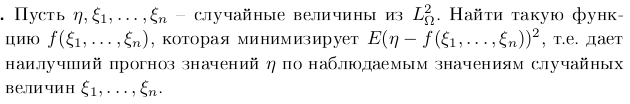
\includegraphics[width=\textwidth]{27.png}
	\end{center}
	}
	\solution{~}
	\section{Многомероное нормальное распределение}
	\problem{~
	\begin{center} 
	    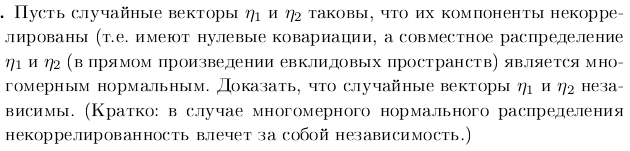
\includegraphics[width=\textwidth]{28.png}
	\end{center}
	}
	\solution{~}
	\problem{~
	\begin{center} 
	    
\includegraphics[width=\textwidth]{29.png}
	\end{center}
	}
	\solution{~}
\end{document}